\documentclass[letterpaper,12pt]{article}

\ifdefined\ungated
\else
\def\ungated{1}
\fi
\ifdefined\submission
\else
  \def\submission{0}
\fi

\usepackage{amssymb,datetime,xspace,amsfonts,amsmath,amsthm,scalefnt,wrapfig,graphicx,subfigure,pdflscape,natbib,multirow,longtable,array,rotating,bibunits,fix-cm,float,epsfig,epstopdf,refstyle,tabularx,booktabs,tikz,verbatim,bbm}
\usepackage[shortlabels]{enumitem}
% \usepackage[american]{babel}
\usepackage[flushleft]{threeparttable}

\usepackage[margin=1in]{geometry}

\usepackage{url}
\usepackage{pdfpages}
\usepackage[libertine]{newtxmath}
\usepackage{libertine}
\graphicspath{{../Images/}}
\newcommand{\alert}[1]{{\color{red}#1}}
\definecolor{mDarkTeal}{HTML}{23373b}
\usepackage[normalem]{ulem}

\epstopdfsetup{suffix=}
\setcounter{MaxMatrixCols}{10}
\usetikzlibrary{matrix,shapes,arrows}
%\pgfkeys{/pgf/number format/.cd,fixed,fixed zerofill,precision=2}
\usepackage{afterpage}
\usepackage{eurosym}
\usetikzlibrary{arrows,positioning,decorations.pathreplacing} 
\usetikzlibrary{shapes.misc, positioning}
\usetikzlibrary{shapes.geometric}

\newtheorem{theorem}{Theorem}
\newtheorem{acknowledgement}[theorem]{Acknowledgement}
\newtheorem{algorithm}[theorem]{Algorithm}
\newtheorem{axiom}[theorem]{Axiom}
\newtheorem{case}[theorem]{Case}
\newtheorem{claim}[theorem]{Claim}
\newtheorem{conclusion}[theorem]{Conclusion}
\newtheorem{condition}[theorem]{Condition}
\newtheorem{conjecture}[theorem]{Conjecture}
\newtheorem{corollary}[theorem]{Corollary}
\newtheorem{criterion}[theorem]{Criterion}
\newtheorem{definition}[theorem]{Definition}
\newtheorem{example}[theorem]{Example}
\newtheorem{exercise}[theorem]{Exercise}
\newtheorem{lemma}[theorem]{Lemma}
\newtheorem{notation}[theorem]{Notation}
\newtheorem{problem}[theorem]{Problem}
\newtheorem{implications}{Testable Implications}
\newtheorem*{implications*}{Testable Implications}
\newtheorem{proposition}{Proposition}
\newtheorem{lem}[theorem]{Lemma}
\newtheorem{remark}[theorem]{Remark}
\newtheorem{solution}[theorem]{Solution}
\newtheorem{summary}[theorem]{Summary}
\def\defeq{\mathrel{\mathop:}=}
\usepackage{setspace}
\usepackage[makeroom]{cancel}

%\setlength{\belowdisplayskip}{3pt}

\newcommand{\ex}[2][{}]{\mathbb{E}_{#1}\left[ #2 \right]}
\newcommand{\Epsi}{\mathcal{E}}
\newcommand{\wt}[1]{\widetilde{#1}}
\newcommand{\wh}[1]{\widehat{#1}}
\newcommand{\wb}[1]{\overline{#1}}
\newcommand{\tteal}[1]{\textcolor{teal}{#1}}
\renewcommand{\baselinestretch}{1.0}
\newcommand{\eur}{\text{\euro}}
% \setlength{\skip\footins}{0.8\baselineskip}
% \setlength{\footnotesep}{0.5\baselineskip}
%\newcommand{\ind}[1]{\index{#1@\emph{#1}}}
\def\ind{\mathbbm{1}}

\usepackage{hyperref}
\hypersetup{allbordercolors={1 1 1},allcolors=blue!65!black,colorlinks=true}
\usepackage[space]{grffile}
\usepackage[bf,small]{caption}
\usepackage[capitalize,nameinlink]{cleveref}

\newcolumntype{C}[1]{>{\centering\arraybackslash}p{#1}}
\usetikzlibrary{arrows,positioning,decorations.pathreplacing} 

\tikzset{
    >=stealth',
    %Define boxe
    punkt/.style={
           rectangle,
           rounded corners,
           draw=black, thick,
           text width=18em,
           minimum height=2em,
           align=flush left},
    % Define arrow
    pil/.style={
           -,
           thick,
           shorten <=2pt,
           shorten >=2pt,}
}

\newcommand{\mycr}[1]{%
  \tikz[baseline=(char.base)]\node[anchor=south west, draw,rectangle, rounded corners, inner sep=2pt, minimum size=4mm,
    text height=1.5mm](char){\ensuremath{#1}} ;}
		
\definecolor{forestgreen}{rgb}{0.0, 0.27, 0.13}

\allowdisplaybreaks

\newenvironment{figurenotes}[1][Note]%
{\small \emph{#1: }}%
{}%

\newenvironment{tablenotes1}[1][Note]%
{~\\\small \emph{#1: }}%
{}%

\bibliographystyle{style1}

\def\acknotitle{Thanks for insightful discussions to Anmol Bhandari, Martin Beraja, Gita Gopinath, Lars Peter Hansen, Juan Carlos Hatchondo, Julian Kozlowski, Leonardo Martinez, Andy Neumeyer, Juan Passadore, Ignacio Presno, Juan Sánchez, Thomas Sargent, Nicholas Trachter, Jeromin Zettelmeyer, and the participants at several academic seminars and conferences. The views expressed in this paper are those of the authors and do not necessarily represent those of the IMF, its Executive Board, or management.}


\title{Uncertainty Premia, Sovereign Default Risk, and State-Contingent Debt\thanks{\acknotitle}}

\author{
\href{https://sites.google.com/site/franroch/}{\color{mDarkTeal}Francisco Roch}\\{IMF \& UTDT}
\and
\href{https://fqroldan.github.io}{\color{mDarkTeal}Francisco Roldán}\\{ IMF}
}

\date{%
\monthname\xspace \the\year%
}

\begin{document}

\fontsize{12.0pt}{25.0pt} \selectfont

\ifnum\ungated=1%
  \maketitle
  \begin{abstract}
  \noindent%
  \fontsize{12.0pt}{18.0pt}\selectfont%
  \input{abstract_sci.txt}
  \end{abstract}
  \renewcommand{\thefootnote}{\fnsymbol{footnote}} \renewcommand{%
  \thefootnote}{\arabic{footnote}} %\fontsize{11}{15}\selectfont
  \thispagestyle{empty} \setcounter{page}{0}
  \fontsize{12.0pt}{25.0pt} \selectfont
  \vfill
  \noindent\textbf{JEL Classification} \quad E43, E44, F34, G12, H63, O16 \\
  \noindent\textbf{Keywords} \quad Sovereign debt, default risk, state-contingent debt instruments, robust control, ambiguity premia
  \vfill
\else
  \includepdf[pages=-]{cover_imfwp_sci.pdf}
  \tableofcontents
\fi


\newpage

\ifdefined\ungated
\else
	\def\ungated{1}
\fi

\ifnum\submission=1%
\else
  \section{Introduction}
\fi

The recent European sovereign debt crises and the increase in public debt levels after the COVID-19 shock have brought proposals for state-contingent debt instruments to the forefront of policy debates as a strategy to avoid costly defaults (\citealp{UN2006}; \citealp{Blanchard2016}; \citealp{IMFpolicy2017}; \citealp{IMF2020}). There is also a substantial theoretical literature focusing on the merits of indexing sovereign debt to real variables to help with macroeconomic stabilization and risk sharing. \cite{Shillerbook}, \cite{HMindexed2012}, \citet*{voxeubook} and \cite{KimOstry2021} argue that GDP-indexed bonds could allow governments to reduce both the cyclicality of fiscal policy and default risk while improving risk sharing with international creditors. More generally, the benefits of improving international risk sharing have been discussed extensively since the seminal work by \cite{BackusKehoeKydland92}. Several recent studies focusing on the advantages of fiscal unions have found that the gains from improving regional stabilization and risk sharing are quantitatively important (\citealp{Beraja2020}; \citealp{FarhiWerning2017}). \cite{ObstfeldPeri1998} argue that state-contingent debt could replicate these features without having to resort to a politically unfeasible combination of taxes and transfers.\footnote{\cite{Beraja2020} and \cite{FarhiWerning2017} show that the efficient risk sharing arrangement within a fiscal union could be achieved through a simple contingent transfer rule that bear resemblances to a GDP-indexed bond.}

Despite these well-understood advantages, the use of state-contingent debt instruments is scarce in practice and countries have not been able to issue such financial instruments at a reasonable premium---as in the recent cases of Argentina (2005), Greece (2012) and Ukraine (2015). Surprisingly, while some practical implementation challenges have been discussed among policy makers, there is little theoretical analysis investigating them and the lack of indexation in sovereign debt markets remains a puzzle. \citet{IMFpolicy2017} and \citet{voxeubook} point to myopia on the part of issuers, who might be out of office before the gains fully materialize.\footnote{\cite{Amador2012} and \cite{AguiarAmadorFourakis2020} study sovereign debt models including political myopia that could arise because of political polarization or political turnover.} \cite{Krugman88} argues that GDP-indexed bonds could create moral hazard problems by deincentivizing the government to conduct growth-friendly policies or misreport GDP statistics. However, these arguments do not seem to be empirically relevant.\footnote{This argument should also apply to inflation-linked bonds but many countries have issued these type of securities. Moreover, the moral hazard problem could also apply to non-contingent debt if the costs of defaults vary with income as is often assumed in the sovereign default literature.} Others argue that markets for these instruments tend to be shallow and, thus, these bonds would carry a large liquidity premium. \cite{Moretti2020} investigates this liquidity channel and finds that state-contingent debt is still welfare-improving. Overall, there are no compelling arguments in the literature to outweigh the aforementioned merits of indexation and justify their little use in practice.

This paper aims to fill this gap and proposes a novel mechanism to understand why state-contingent debt has only been issued on a modest scale and severely underpriced. We evaluate state-contingent instruments in light of a sovereign default framework à la \cite{Eaton81} with long-term debt, augmented with international lenders who fear model misspecification.\footnote{\cite{JIE} show that allowing for long-term debt introduces a time inconsistency problem (debt dilution) that improves the quantitative performance of sovereign default models. If the government only issues one-period bonds, there is no time inconsistency in borrowing decisions (\citealp{AguiarAmador2019}).} Since the seminal contribution of \citet{Arellano05}, the Eaton-Gersovitz model has been widely used in studies of fiscal policy for countries with default risk. In our environment, foreign lenders have doubts about the probability model of the small open economy's exogenous income process and guard themselves against this ambiguity by forming pessimistic expectations. Lenders with preferences for robustness distort probabilities about exogenous shocks in an endogenous way by boosting the probability of low-utility states and seek decision rules that perform well under these worst-case distributions. In the model, low utility events are associated with periods of high default risk and, in the case of state-contingent debt, periods in which stipulated repayments are low.

The presence of robust lenders creates a tradeoff for the optimal design of state-contingent debt. Obtaining more insurance from lenders increases the relevance of their doubts about the true stochastic process governing the indexing variable. On the other hand, contingency in stipulated repayments can help reduce the probability of default and the volatility of consumption while improving risk sharing with the foreign creditors as in previous studies \citep[e.g.,][]{HMindexed2012}. The typical design of state-contingent instruments that countries have recently used involves a threshold below which no payments are made (Argentina 2005, Greece 2012, and Ukraine 2015 are 21st century examples). This threshold structure, especially when the threshold is imposed at relatively high levels of income, is sensitive to the types of probability distortions that robust lenders worry about, which leads them to heavily discount the bond.\footnote{In contrast, many countries implicitly index their debt portfolio through a combination of local-currency, foreign-currency, and inflation-indexed debt, which builds in state-contingency but avoids thresholds. Low spreads in such cases is consistent with our model, where linear indexation is generally superior to threshold indexation.} Threshold indexation also provides little insurance in exchange for the repayment variance it imposes on lenders. In line with the empirical evidence, our model with robust lenders generates wide spreads for this threshold-type of instruments, which also lead to equilibrium welfare losses compared to noncontingent debt and, thus, explains why governments seem so reluctant to issue these instruments.

Robustness is a standard device in the asset-pricing literature which enables more realistic market prices of risk. In the context of noncontingent debt, \cite{PouzoPresno2016} show that augmenting the baseline sovereign default model with robust lenders is essential to simultaneously match the spread dynamics and the frequency of default observed in the data. They also show that the same model with lenders with standard CRRA preferences and no robustness would generate counterfactually high bond prices for plausible levels of risk aversion. Similarly to the equity premium puzzle, for large values of risk aversion the model without robustness can generate high spreads for noncontingent debt at the expense of an extremely low risk-free rate at odds with the data.

We motivate this framework as a way to capture concerns that the model used to fit the past GDP series, or the underlying variable associated with the state-contingent bond, does not (yet) accurately capture all relevant features of the economy. While we do not pursue them, there are other reasons why the robust-lenders model can be appealing. One is that robustness captures potential concerns that the evolution of the country's GDP may be different in the future than the current estimate of what it has been in the past. It could be that, as a result of (the success of) moving to state-contingent debt, the government modifies its fiscal or monetary policies. It could even be that reported GDP and actual GDP diverge because of incentives to misreport statistics. Finally, it could be that issuing state-contingent debt signals some underlying type of the government: maybe an impatient one who seeks to finance irresponsible policies, or a responsible one who seeks to improve risk-sharing with the rest of the world. While we would prefer explicit models of most of these features, robustness could in principle be interpreted as representing some of them, informally capturing the degree of credibility that lenders assign to the countries they lend to.

The sovereign default framework à la \cite{Eaton81} is commonly used for quantitative studies of sovereign debt and has been shown to generate a plausible behavior of sovereign debt and spreads. Formally, we analyze a small open economy that receives stochastic endowments of a single tradable good. The government is benevolent, issues long-term debt in international markets, and cannot commit to repay its debt. While not in default, the government issues debt which is purchased and priced by competitive foreign lenders. Following \cite{PouzoPresno2016}, we extend the canonical model by assuming that these foreign lenders are endowed with multiplier preferences \citep{HansenSargent2001}, a tractable way to introduce concerns for robustness. In our baseline model, the government issues noncontingent bonds. By varying the asset structure, we examine the equilibrium consequences of making debt payments linked to the realization of the income shock in different ways.

We structure our discussion around the GDP warrants issued by Argentina as part of its 2005 debt restructuring.  \citet*{ChamonCostaRicci2008} find that these bonds traded at large premia: around 300bps which they attribute to the default risk of other securities, and a residual of between 600 and 1200bps which they interpret as a premium for `novelty.' We first calibrate our model to match key moments in the data for Argentina assuming that the government only issues noncontingent debt. Then we evaluate the effects of indexation by assuming the government can issue a state-contingent bond (which we label as `threshold' bond) that resembles the structure of the GDP warrant issued by Argentina. With rational-expectations lenders, this threshold bond provides welfare gains to the country relative to noncontingent debt. The threshold bond also realizes about two-thirds of the welfare gains of optimal state-contingent debt when facing rational-expectations lenders. These welfare gains, however, are overturned with robust lenders, who charge high spreads as their probability distortions magnify the likelihood of states with lower payments---an ambiguity spread. This ambiguity spread explains most of the so-called novelty premium on Argentine GDP warrants and, more broadly, the lack of appetite for issuing these instruments.

We then characterize the structure of the optimal state-contingent bond and show how it is affected by the degree of robustness.  In contrast to the commonly used threshold bond, the optimal design generates substantial welfare gains, although these gains are decreasing in the level of robustness. For tractability, we first characterize the optimal design of state-contingent debt in a stylized version of our model. We show how mean-preserving differences in the structure of promised repayments --which have no impact on rational-expectations, risk-neutral lenders-- may imply large differences in the spreads charged by lenders who fear model misspecification. The lenders' robustness limits the scope for risk-sharing in particular ways: the optimal debt structure features less contingency, lower slopes, and an avoidance of regions with zero or low stipulated repayments. For a given level of insurance, the government would like to minimize the contingency in stipulated repayments in order to prevent costly probability distortions. But the degree of hedging it can attain is itself limited by default risk ex-post.\footnote{\citet*{DvorkinSanchezSaprizaYurdagul} argue that restructurings introduce some state-contingency ex-post.} As the insurance-cost schedule moves out with robustness, welfare gains from optimal state-contingent are decreasing in the degree of robustness. These insights are preserved in the quantitative version of our model, where for computational reasons we only optimize over a parametric family of state-contingent instruments.

Overall, our findings cast doubts about the desirability of using the threshold type of state-contingent bonds that countries have been issuing in the past and demonstrate how the optimal bond indexation depends on the degree of lenders' preferences for robustness. Our model rationalizes the so-called novelty premia in threshold bonds as ambiguity premia associated with the type of contingency these bonds introduce. These premia overturn the well-understood advantages of indexed bonds (which are present in our model) and create substantial welfare losses for the government. Robustness can therefore explain why state-contingent bonds with GDP thresholds for repayment have not been generally regarded as successful by their issuing countries.

\paragraph{Discussion of the Literature} Our analysis builds on and extends three branches of the literature: sovereign default, robust control theory, and the implications of state-contingent debt. First, our study is related to the recent literature on quantitative models of sovereign default that extended the approach developed by \cite{Eaton81}, starting with \cite{AG_06} and \cite{Arellano05}. Different aspects of sovereign debt dynamics and default have been analyzed in these quantitative studies. Excellent surveys of the literature on sustainable public debt and sovereign default can be found in \citet*{AguiarAmador2021} and in handbook chapters by \citet{AguiarAmadorHandbook}, \cite*{ACCS}, and \cite*{DerasmoMendozaZhang}.

Our study also relates to the literature on robust control methods pioneered by \cite{HansenSargent2001,HansenSargent2011}. A growing theoretical macro literature extends canonical models to the case in which the social planner and/or private agents fear model misspecification and search for robust policies under worst-case scenarios (\citealp{AdamWoodford2012}, \citealp{Young12}, \citealp{FerriereKarantounias},  \citealp{MontamatRoch}). We relate closely to \cite{PouzoPresno2016} who study a sovereign default model with robust international lenders in the context of noncontingent debt. Their analysis demonstrates how the introduction of robust lenders improves the quantitative performance of sovereign default models. Robustness helps match bond spreads dynamics observed in the data without resorting to counterfactually high default frequency by historical standards. We then study how international investors' concerns about model misspecification affect the spreads, welfare implications, and optimal design of state-contingent bonds. 

Finally, our paper naturally relates to a literature concerned with the implications of state-contingent debt. \cite{BorenszteinMauro2004} focus on the implications and benefits of state-contingent debt for the cyclicality of fiscal policy. \cite{Durdu} shows that the degree of indexation should be optimally chosen to smooth sudden stops, and that this optimal degree of indexation depends on the persistence and volatility of the shocks an economy faces. More closerly related to our paper, \cite{HMindexed2012} and \cite{SandlerisSaprizaTaddei2017} study the effects of introducing income-indexed bonds into standard quantitative sovereign default models. Both studies find that, in models without robustness, GDP-indexed securities support large welfare gains when designed optimally. These papers emphasize that GDP-linked bonds allow the government to eliminate default risk while increasing indebtedness, thereby reducing the equilibrium volatility of consumption relative to income. However, their baseline model with one-period bonds generates counterfactual bond spread dynamics and debt levels. For example, the benchmark calibration in \cite{HMindexed2012} generates a 3\% mean spread and 4\% debt-to-income ratio in their simulations. We build on these papers by clarifying how robustness on the part of lenders helps match empirical (low) bond prices which ultimately overturns the conclusions on welfare implications of state-contingent debt for the designs observed in reality.

\paragraph{Layout} The remainder of the paper is structured as follows. First, section \ref{sec:summarySCI} documents recent country experiences with sovereign state-contingent bonds and motivates the mechanism proposed in the paper. Section \ref{sec:2permodel} lays out a simple two-period model that illustrates how the optimal design of state-contingent bonds and the associated welfare implications depend on the lenders' preferences for robustness. Section \ref{sec:quantmodel} introduces the quantitative model. Section \ref{sec:quantresults} contains our main results on the equilibrium effects of different state-contingent debt instruments. Finally, section \ref{sec:conc} concludes.
 

\section{Recent experiences with state-contingent debt and the case for robustness \label{sec:summarySCI}}

State-contingent debt instruments are not used frequently in sovereign borrowing. Subsection \ref{subsec:summarySCI_1} summarizes some recent cases, along with a description of the contingency involved in the various issuances, and shows that these bonds have traded at a large premia. Subsection \ref{subsec:summarySCI_2} discusses why we consider that robustness provides a better rationale for this underpricing over alternative explanations in the literature.

\subsection{The design of state-contingent debt and the `novelty' premium \label{subsec:summarySCI_1}}

\citet*{databaseSCI} compiles 38 instances of issuances of sovereign state-contingent debt, ranging from cotton bonds issued by the Confederate States of America in 1863 to the IBRD Cat bonds issued in 2018 by Peru, Colombia, Chile, and Mexico to stipulate lower debt payments in case of earthquakes. The vast majority of bonds are structured in a way that promises reduced or no payments if some measure of income (such as output or a key export price, among others) falls below a certain threshold. 

\citet*{ChamonCostaRicci2008} describe in detail the GDP-warrants issued by Argentina as part of its 2005 debt restructuring. This contract was characterized by a threshold and a slope. Payments only occured if the state of the economy satisfied three conditions. First, real GDP growth must exceed `baseline' GDP growth in the reference year.\footnote{Baseline GDP growth was set by the authorities to gradually converge from an initial level of $4.3\%$ in 2005 to a long-run level of $3\%$ at the maturity of the bond in 2034.} Second, the level of real GDP had to be higher than the compounding of the baseline growth rates. Finally, payments only occured if the cumulative amount of past payments was below another threshold (of $48$ cents of the currency of denomination per unit of security). If the threshold was satisfied, the slope component of the bond meant that payments were a fraction of the difference between the actual and baseline levels of real GDP. \citet*{ChamonCostaRicci2008} use Monte Carlo simulations based on historical data to compute theoretical prices for the GDP warrants from 2005 to 2007. They find wide spreads: between 300 and 400bps which they attribute to the default risk of other securities, and a residual of 1200bps (which declined over time to about 600bps) which they interpret as a premium for `novelty.'

The decline in the residual premium featured in \citet*{ChamonCostaRicci2008} could indeed justify labeling it as `novelty' implying that these were relatively exotic assets and, thus, market participants needed time become familiar with the trading of these state-contingent bonds. Moreover, the severe underpricing could also be related to a poor economic outlook specific to Argentina, given its fragile macroeconomic framework. However, \cite{Taehoon} update the exercise in \citet*{ChamonCostaRicci2008} with more recent data (also extending to additional countries), and their results suggest otherwise. Figure \ref{Figures_Taehoon} shows the estimated spread decomposition for the GDP-warrant issued by Argentina, Greece and Ukraine. The residual premium, which they label as `SCDI Premium,' has remained at a high level in the case of Argentina over a period of 15 years. They also find a significant residual premium in the recent issuances by Greece and Ukraine. These results indicate that the underpricing of these instruments is not a country-specific issue and does not seem to be related to the novelty of the instrument.

\begin{figure}[!hbtp]
	\includegraphics[width=0.495\textwidth]{fig2_arg.eps}
	\includegraphics[width=0.495\textwidth]{fig2_grc.eps}
	\begin{center}
		\includegraphics[width=0.5\textwidth]{fig2_ukr.eps}
	\end{center}
	\caption{GDP-linked security premia. \label{Figures_Taehoon}}
	\begin{figurenotes}
	The figure shows the estimated spread decomposition in \cite{Taehoon} for the GDP-warrants issued by Argentina (top left), Greece (top right) and Ukraine (bottom). 
	\end{figurenotes}
\end{figure}

\subsection{Why robustness? \label{subsec:summarySCI_2}}

Among the existing arguments for the lack of indexation in sovereign debt markets discussed in the Introduction, concerns about data accuracy and moral hazard related to misreporting statistics seem to be the most shared in policy circles. However, these concerns should not be overemphasized. First, these arguments should also apply to inflation-linked bonds which many countries have managed to trade a reasonable prices.\footnote{Notice that inflation-linked bonds typically do not involve repayment thresholds.} Second, in the case of GDP-linked bonds, governments would pay significant political costs for underreporting growth. Moreover, long maturities could correct for the moral hazard problem, as the GDP growth rate would be less manipulable over the longer term. In fact, in the case of Argentina, the government has been criticized for allegedly \emph{over}reporting growth and underreporting inflation. In the case of Greece, the issuance of GDP-linked securities occurred under the scrutiny of the European Commission, the ECB and the IMF. The oversight of these international organizations reduces the margin for data inaccuracies or misreporting, but nevertheless the Greek GDP-linked warrants were also heavily discounted (see Figure \ref{Figures_Taehoon}).

The theoretical values for the Argentina GDP-warrant estimated in \citet*{ChamonCostaRicci2008} were significantly above those in market reports. This valuation discrepancy was mainly related to the assumptions regarding the growth process. While their calculations were based on the average of the Consensus Forecast, \citet*{ChamonCostaRicci2008} also state that investment banks’ pricing models exhibited more conservative growth forecasts. This suggests that investors’ forecasts of GDP growth were in general pessimistic and underpredicted Argentina's economic recovery. Finally, \citet{CantorPacker1996} argues that financial markets regard sovereign ratings with skepticism, and \citet{GrossePodstawski2017} provide some more recent evidence of investor pessimism and ambiguity-aversion in sovereign debt markets, in line with \citet{PouzoPresno2016}.

Our framework with robustness captures investors' pessimism when pricing sovereign debt. The discrepancy in growth forecasts reflects that investors have not settled on a `true' model governing the data and/or are concerned about specification errors behind the processes used to model economic variables.\footnote{As mentioned before, our framework could also be reinterpreted to accommodate concerns about data reliability and misreporting. If potential misreporting drives a wedge between reported and actual data, reported data could be conceptualized as being generated by a perturbation of the statistical process governing actual data. External scrutiny and other forces discussed above would limit the size of this perturbation, which in our framework maps into a cap on the contribution of these sources to the overall robustness parameter.} Thus, robust lenders charge an uncertainty premium by slanting probabilities towards worse but plausible scenarios to guard themselves against possible errors in the estimated process.

%provides support for our robust lenders who would charge an uncertainty premium by slanting probabilities towards worse but plausible scenarios. %Moreover, modelling lenders who fear model misspecification also captures the potential concerns about data reliability and misreporting discussed above.



%As was the case with other similar instruments, the Argentinian GDP warrants traded at heavy discounts. Pricing bonds with indexed repayments requires taking expectations and therefore a model for the distribution of the stochastic process upon which the payments are contingent. \citet*{ChamonCostaRicci2008} use Monte Carlo simulations based on historical data to compute theoretical prices for the GDP warrants we are interested in. They find wide spreads: between 300 and 400bps which they attribute to the default risk of other securities, and a residual of 1200bps (which declined over time to about 600bps) which they interpret as a premium for `novelty.' As we will see below, our framework with robust lenders is able to generate deep discounts, in line with the empirical evidence. In this sense, we interpret the wide spreads on some types of sovereign state-contingent debt as reflecting ambiguity premia.



\section{A stylized model of sovereign default with robustness \label{sec:2permodel}}

This section presents a stylized sovereign default model to conceptually explore the interaction between state-contingent debt and robustness. A small open economy, populated by a government and a representative agent, faces risk-neutral competitive foreign lenders. The world lasts for two periods in which the government receives endowments $(y_1, y_2)>0$. There is uncertainty about $z$ which determines the value of income in the second period $y_2(z)$.

\paragraph{Assets} Only one type of security is traded.\footnote{In line with previous studies \citep{BorenszteinMauro2004, Durdu, HMindexed2012, HMSP16, SandlerisSaprizaTaddei2017, KimOstry2021, SosaPadillaStruzenegger2021}, we abstract from the portfolio problem and compare the cases of noncontingent and contingent debt.}
When the government issues debt, it promises a repayment $R(z)$ in state $z$ of the second period. Different specifications of the stipulated repayment function $R$ represent different types of state-contingent debt structures. We focus on four different types of repayment functions summarized in Table \ref{tab:R(z)}.

\begin{table}[!hbtp]\centering \small
\caption{Stipulated repayment functions}\label{tab:R(z)}
\begin{tabular}{@{}lccc@{}}\toprule
  \textbf{Type of debt} & \multicolumn{3}{c}{\textbf{Stipulated repayment}} \\\midrule
  Noncontingent debt & $R(z)$ & $ = $ & $1$ \\
  Linear indexing & $R^\alpha(z)$ & $ = $ & $1 + \alpha \left( y_2(z) - \mathbb{E}_1\left[y_2(z)\right] \right) $ \\
  Threshold debt & $R^\tau(z)$ & $ = $ & $\ind\left(y_2(z) > \tau\right)$ \\
  Optimal design & $R^\star(z; \theta)$&       & {\footnotesize chosen state by state}\\\bottomrule
\end{tabular}
\end{table}
Noncontingent debt promises a constant repayment regardless of the state, while the repayment of linearly-indexed debt depends on the difference between realized output and its mean, with a slope parameter of $\alpha \geq 0$.\footnote{In the model, we use $\max\{0,R^\alpha(z)\}$ when considering linearly-indexed debt to keep repayments nonnegative. We skip the $\max$ in the description to keep the notation succint.} Threshold debt pays only if the state is above a minimum level. Finally, we compute the debt structure that maximizes the utility of the government by promising non-negative repayments $R^\star$ state-by-state in a flexible manner. Our notation anticipates that the optimal design depends on the lenders' preferences as summarized by the robustness parameter $\theta$ introduced below.

\paragraph{Government} The government is benevolent and makes decisions on a sequential basis. The government acting in period $j \in \{1,2\}$ maximizes $\mathbb{E} \left[ \sum_{t=j}^2 \beta_b^{t-j} u\left( c_t \right)\right]$, where $\mathbb{E}$ denotes the expectation operator, $\beta_b \in (0,1]$ is the government's discount factor, $c_{t}$ represents period-$t$ consumption in the economy, and the utility function $u$ is increasing and concave. The government borrows to finance consumption in period 1, taking as given the stipulated repayment function $R$. The government may choose to default in period 2, in which case it does not pay the debt but loses $\phi(z)$ of the endowment $y_2$. We consider a standard quadratic specification for the output-cost function, meant to make the cost of default increasing and convex in output
\begin{align*}
  \phi(z) =  d_1 y_2(z)^2
\end{align*}

The government understands the pricing function $q(b)$ that foreign lenders offer for an issuance level $b$. For ease of notation, we omit the dependence of $q$ on $R$ and $\theta$. The government's problem is to choose debt and consumption to solve
\begin{align*}
	V(\theta, R) = &\max_b u(c_1^b) + \beta_b \mathbb{E}\left[u(c_2^b) \right] \\
	\text{subject to }\;
	& c_1^b = y_1 + q(b) b \\
	& c_2^b = y_2(z) - \phi(z)d(b,z) - (1-d(b,z)) R(z) b
\end{align*}
where $d(b,z)$ takes the value of 1 if the goverment defaults in state $(b,z)$ and 0 otherwise. $V(\theta, R)$ denotes the equilibrium value attained by the government when it faces lenders with robustness $\theta$ and issues debt with stipulated repayment $R$. It is common knowledge that default takes place if and only if
\begin{align*}
	u\left(y_2(z) - \phi(z)\right) > u\left(y_2(z) - R(z) b\right)
\end{align*}

\paragraph{Lenders} We focus on the interaction between the design of the debt instrument and the lenders' degree of robustness. Following \citet{HansenSargent2001} and \citet{PouzoPresno2016}, we assume that foreign lenders feature \emph{multiplier preferences} to capture concerns about potential model misspecification. Multiplier preferences lead our lenders to price assets by distorting their approximating or benchmark model.\footnote{\citet{PouzoPresno2016} provide a thorough discussion of robustness in the context of sovereign debt models.}

Standard arguments from the robustness literature allow us to write the lenders' problem as\footnote{See Appendix \ref{app:lenders}.}
\begin{align*}
	&\max u(c_1^L) - \frac{\beta}{\theta} \log \left( \mathbb{E}\left[ \exp(-\theta v_2^L) \right] \right) \\
	\text{subject to }\;
	& v_2^L = u(c_2^L) \\
	& c_2^L = w_2 + (1-d(b,z)) R(z) b \\
	& c_1^L = w_1 - q(b) b
\end{align*}
where $(w_1, w_2)$ are the lenders' endowments in periods 1 and 2, respectively.\footnote{If lenders are risk-neutral, the relative size of their endowment $(w_1, w_2)$ is irrelevant for outcomes \citep[see][for a proof in the context of noncontingent debt]{PouzoPresno2016}. In the case of risk-averse lenders, the relative size of their endowments can also be important in shaping their risk-appetite. Moreover, in general, lenders can be affected by developments in the economy through a correlation between these quantities and the endowment shocks.}

The lenders' first-order conditions yield a pricing equation for the debt
\begin{align*}
	u'(c_1^L) q(b) = \beta \mathbb{E}\left[ \frac{\exp(-\theta u(c_2^L))}{\mathbb{E}\left[\exp(-\theta u(c_2^L))\right]} u'(c_2^L) (1-d(b,z)) R(z) \right]
\end{align*}
where $M = \beta \frac{\exp(-\theta u(c_2^L))}{\mathbb{E}\left[\exp(-\theta u(c_2^L))\right]}$ augments the stochastic discount factor. The parameter $\theta$ controls the degree of ambiguity aversion. This Euler equation makes it clear that the model converges back to expected utility with rational expectations as $\theta \to 0$. In our baseline, lenders have per-period payoff linear in consumption, while also being uncertainty averse or ambiguity averse.\footnote{We leave the lenders' utility function general, even though we focus on the risk-neutral case. In general, it can be jointly calibrated along with the robustness parameter $\theta$ to match asset-pricing evidence. Another alternative is to calibrate $\theta$ to a reasonable model error-detection probability.}


\paragraph{Ambiguity premia} The robust-lenders model links bond prices and spreads to features of equilibrium expectations about debt repayment. For risk-neutral (but still robust) lenders, we have
\begin{align}\label{eq:Euler_decomp}
  q(b; R, \theta) &= \beta \mathbb{E}\left[ \frac{\exp(-\theta c_2^L)}{\mathbb{E}\left[\exp(-\theta c_2^L)\right]} (1-d(b,z)) R(z) \right] \notag \\
  &= \underbrace{\beta \mathbb{E}\left[(1-d)R\right]}_{=\, q_{\text{\emph{RE}}}} + \underbrace{\left(1-\mathbb{P}(d)\right)\text{cov}{(M,R)}}_{=\, q_\theta^\text{\emph{cont}}} - \underbrace{\mathbb{E}\left[R\right]\text{cov}{(M,d)}}_{=\, q_\theta^\text{\emph{def}}}
\end{align}

Equation (\ref{eq:Euler_decomp}) breaks up the debt price into a rational-expectations component $q_\text{\emph{RE}}$ and two components that depend on the degree of robustness. The first of them, $q_\theta^\text{\emph{cont}}$, reflects ambiguity in the contingency of the debt contract itself: given the repayment probability, it is proportional to the covariance between the stochastic discount factor $M$ and the stipulated repayment $R$. The second one, $q_\theta^\text{\emph{def}}$, reflects ambiguity in the default strategy: controlling for the average level of stipulated payments, it is proportional to the covariance between the stochastic discount factor and the repayment strategy. Because the lenders' marginal utility is decreasing in debt payments, these covariances will be respectively negative and positive. Both ambiguity terms contribute to lower bond prices and larger spreads.

We compute and decompose spreads as follows. Let $r = \frac{\mathbb{E}[R]}{q}$ be the implicit interest rate and $r-r^\star$ be the spread, where $r^\star = 1/\beta - 1$ is the international risk-free rate. We define the rational-expectations spread as $\text{\emph{spr}}_\text{RE} = \frac{\mathbb{E}[R]}{q_\text{RE}} - r^\star$, the premium from the ambiguity of contingent repayment as $\text{\emph{spr}}_\theta^\text{\emph{cont}} = \frac{\mathbb{E}[R]}{q_\text{RE} + q_\theta^\text{\emph{cont}}} - \frac{\mathbb{E}[R]}{q_\text{RE}}$, and the premium from the ambiguity of default as $\text{\emph{spr}}_\theta^\text{\emph{def}} = \frac{\ex{R}}{q_\text{RE}+q_\theta^\text{\emph{cont}}+q_\theta^\text{\emph{def}}} - \frac{\ex{R}}{q_\text{RE}+q_\theta^\text{\emph{cont}}}$.

The robust-lenders model allows us to characterize the probability distortions that underpin debt prices in an equilibrium. Let the \emph{distorted expectation} of a random variable $X$ be the objective expectation of the product of $X$ with a likelihood ratio
\begin{align}\label{eq:kernel}
  \tilde{\mathbb{E}}\left[X\right] = \mathbb{E}\left[\frac{\exp(-\theta u(c_2^L))}{\mathbb{E}\left[\exp(-\theta u(c_2^L))\right]} X \right]
\end{align}
As compared to the expectation taken with the objective probability measure, the distorted expectation magnifies the likelihood of states for which the lenders' utility is low. Different designs for government debt (different $R$ functions) lead to different equilibrium outcomes for lenders, which in turn support different worst-case models and different probability distortions.

\subsection{Probability Distortions}
To investigate the effect of robustness on state-contingent debt prices, we solve the stylized model for different repayment functions $R$ and different levels of the robustness parameter $\theta$. We leverage Equation (\ref{eq:kernel}) to recover the probability distortions used by lenders to evaluate debt payoffs in each equilibrium.

Table \ref{Table_2per_parameters} summarizes our parametrization. We keep close to the Argentinian GDP-linked bonds described in \citet*{ChamonCostaRicci2008}. The parametrization is purposely artificial to highlight how the lenders' robustness interacts with the design of bonds to create spreads. 
In particular, we allow the robustness parameter $\theta$ to vary between $0$ (rational expectations) and $4$, an arbitrary level that is high enough to illustrate the forces at play. Section \ref{sec:quantmodel} focuses on an infinite-horizon version of the model calibrated to Argentina in which $\theta$ is controlled by model detection error probabilities.
\begin{table}[!hbtp]\centering \small
  \caption{Parametrization of stylized model}\label{Table_2per_parameters}
  \begin{tabular}{@{}lcc@{}} \toprule
    \textbf{Parameter} & \textbf{Target} & \textbf{Value} \\ \midrule
    $\beta_b$       & Borrower's discount rate & 6\% ann. \\
    $\beta$         & Risk-free rate & 3\% ann.        \\
    $\gamma$        & Borrower's risk aversion & 2     \\
    $d_1$        & Output cost of default & 20\%    \\
    $g$             & Expected growth rate& 8\% ann.   \\ 
    $\tau$          & Threshold for repayment & 1   \\
    $\sigma_z$      & Std.~deviation of log output & 0.15 \\
    \bottomrule
  \end{tabular}
\end{table}

One period is five years. We set the first period endowment $y_1$ to make $\mathbb{E}[y_2(z)] = 1 = y_1 (1+g)^5$, so that $g$ is the expected growth rate.\footnote{While foreign lenders agree with the second equality, their worst-case model will in general yield a distorted expectation $\tilde{\mathbb{E}}[y_2(z)] < 1$.} The output cost of default $d_1$ as well as expected growth $g$ are set to high values to simultaneously generate high levels of debt and a low default probability, which is complicated in this stylized model by the use of one-period bonds (this difficulty is absent in our quantitative version with long-term debt). Output in the second period $y_2(z) = \exp(\sigma_z z)$ where $z \sim \mathcal{N}(0,1)$. Other parameters are set to standard values in the literature.

We parametrize our threshold bond structure as follows. We set the repayment threshold $\tau$ at the mean of second-period output. This is meant to replicate the fact that the Argentinian GDP-linked bond was designed to pay if output growth was above average. At the time of issuance, the Consensus Forecast for Argentina's GDP growth was about 3\% over the medium-term, which coincides with the bond's main condition for repayment.

\paragraph{Simple state-contingent instruments}
We begin by analyzing equilibrium outcomes associated with noncontingent debt and threshold debt.

Figure \ref{Figure_distorted_noncontingent} shows the probability distortions when the government issues noncontingent bonds. For ease of exposition, we fix the amount of debt issued at the optimal level when $\theta = 0$ (the rational-expectations case), so that the default probability does not vary with the degree of robustness.\footnote{When the government can optimize issuances as a function of $\theta$, as we will see later, it issues less debt as lenders become more robust and charge higher spreads. This moves the default threshold to the left as $\theta$ increases.} This allows us to concentrate on the effect of robustness on prices, without the compensating reaction of the government. The top panel shows the default probability at each state as a dotted line and the distorted density (used by lenders to evaluate payoffs) in solid lines. The bottom panel shows the stipulated payment $R$ as a dashed line and the likelihood ratios $\frac{\exp(-\theta c_2^L)}{\mathbb{E}\left[\exp(-\theta c_2^L)\right]}$ in solid lines. The distorted density used by lenders equals the likelihood ratio times the objective density.
\begin{figure}[!hbtp]\centering
    \includegraphics[width=0.95\textwidth]{distorted_noncontingent_paper.pdf}
\caption{Distorted probabilities when the government issues noncontingent debt (amount fixed at the rational-expectations eq'm level). Top: distorted densities for each $\theta$ and default probability. Bottom: likelihood ratios (distortions) and promised repayments $R(z)$
\label{Figure_distorted_noncontingent}}
\end{figure}

In the case of noncontingent debt, the expected repayment is a step function of the state $z$: the government defaults when income is low. The lenders' stochastic discount factor is therefore also a step function of the state, as marginal utility of lenders is constant (and high) to the left of the default threshold and constant (and low) to the right of it. As the robustness parameter $\theta$ increases, the metaphorical evil agent has more scope to distort probabilities, and does so by assessing the default set as more likely. For higher values of $\theta$, therefore, the expected return of the debt (under the distorted density) is lower and lenders require higher spreads to hold it.
  
Figure \ref{Figure_distorted_threshold} considers the case of the threshold bond which promises to repay 1 unit of the good if the state is above its mean (under the approximating model which is shared by government, lenders, and Nature) and 0 otherwise. 
\begin{figure}[!hbtp]\centering
  \includegraphics[width=0.95\textwidth]{distorted_threshold_paper.pdf}
\caption{Distorted probabilities when the government issues the threshold bond (amount fixed at the rational-expectations eq'm level). Top: distorted densities for each $\theta$ and default probability. Bottom: likelihood ratios (distortions) and promised repayments $R(z)$
\label{Figure_distorted_threshold}}
\end{figure}
In this case, the probability distortions are much more striking. Similarly to the default threshold, the jump in stipulated repayments creates a jump in the probability distortions. But the same distortion applied to an event with higher probability results in a larger change in the density. Moreover, as we will see later, the large distortions evident in Figure \ref{Figure_distorted_threshold} manifest as high spreads that negate the gains from contingency in repayment.

\paragraph{Optimal debt design} We turn our attention to the problem of how to design state-contingent debt instruments and how the optimal design changes with the degree of robustness. When facing lenders with robustness parameter $\theta$, let $R^\star(z;\theta)$ maximize the equilibrium value attained by the government $V(\theta, R)$, subject to a non-negativity constraint.

Figure \ref{Figure_arrow} shows the optimal debt design $R^\star(z;\theta) = \arg\max_R V(\theta,R)$ for each value of the robustness parameter $\theta$, as well as the expected repayment of noncontingent debt (taking default into account). It is clear that, as $\theta$ increases, the optimal debt structure features less contingency, lower slopes, and an avoidance of regions with zero or low stipulated repayments.
\begin{figure}[!hbtp]\centering
    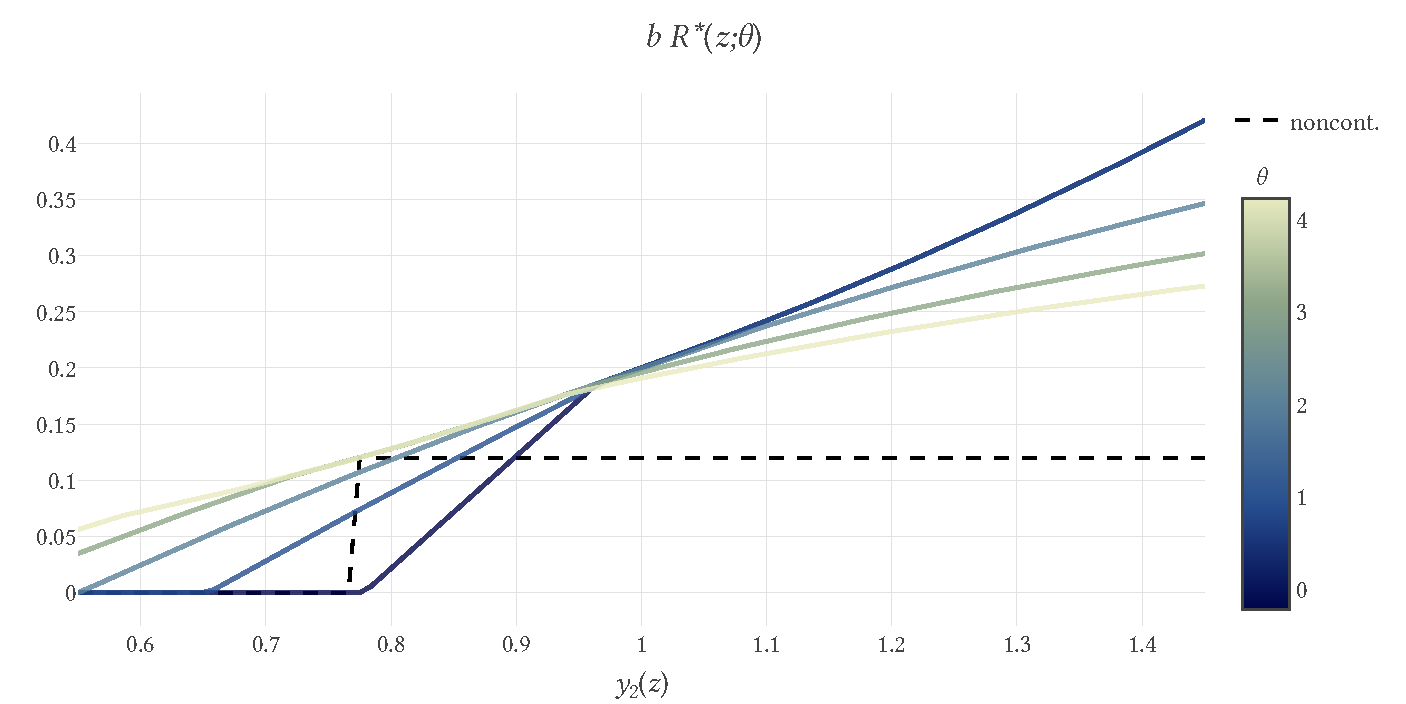
\includegraphics[width=0.9\textwidth]{arrow_paper.pdf}
\caption{Optimal design of state-contingent debt for each type of lender.
\label{Figure_arrow}}
\end{figure}
Figure \ref{Figure_arrow} sharply illustrates the tradeoffs in the debt-design problem when facing robust lenders. On the one hand, the government would like to minimize the contingency in stipulated repayments in order to prevent probability distortions. But the government also needs to minimize another source of contingency given by default risk ex-post. In low states, the government promises as much as it can credibly commit to repay.

\subsection{Spreads}\label{sec:spreads}
We now turn to how the probability distortions and concerns for model misspecification affect bond prices, issuances, and the government's welfare in equilibrium. The top panel of Figure \ref{Figure_spreads_parametric} shows our decomposition of equilibrium spreads as a function of the robustness parameter $\theta$. The bottom panel shows the issuance value $q(b)b$ as well as the welfare of the government. We measure welfare as the equivalent increase in consumption with respect to an equilibrium with the same $\theta$ but when the government issues noncontingent debt.\footnote{Somewhat abusing notation, if
\begin{align*}
  V(\theta, R, x) = u\left(c_1^b(1+x)\right) + \beta \mathbb{E}\left[u\left(c_2^b(1+x)\right)\right]
\end{align*}
is the value attained by the government, augmenting the equilibrium level of consumption by the factor $x$, then in each equilibrium with bonds $R$ and robustness $\theta$ we measure welfare by finding $x$ to make $V(\theta, R, 0) = V(\theta, 1, x)$.}
\begin{figure}[!hbtp]\centering
    \includegraphics[width=1\textwidth]{spreads_parametric_paper.pdf}
\caption{Spreads when the government issues the simple instruments. Bottom panel: issuance value $q(b)b$ and welfare difference from noncontingent debt}\label{Figure_spreads_parametric}
\end{figure}

When the government issues noncontingent debt, more robust lenders charge a higher spread for the ambiguity of default. The government responds by issuing lower amounts of debt. In our parametrization, the decrease in the default probability (the amount of risk) roughly compensates the increase in the spreads because of ambiguity (the price of risk).

Linearly-indexed debt successfully decreases the equilibrium default probability, as evidenced by lower spreads under rational-expectations. This leads to welfare gains equivalent to about $0.9\%$ of consumption from the noncontingent debt benchmark. As robustness increases, spreads from ambiguity of contingency and from ambiguity of default open up, eroding the government's ability to issue debt and therefore welfare gains. At $\theta = 4$, however, the government still values the option to move from noncontingent to linearly-indexed debt at about $0.8\%$ of consumption.

The picture is quite different for threshold debt. This type of debt completely eliminates default risk and therefore trades at no spreads with rational-expectations lenders. However, as $\theta$ increases, the large probability distortions discussed above support large spreads from the ambiguity of contingency. These high spreads quickly turn the welfare gains from state-contingent debt into welfare losses.


\section{The quantitative model \label{sec:quantmodel}}

In this section we present the infinite-horizon version of the two-period model studied in Section \ref{sec:2permodel}. We consider a general formulation in which the government can issue contingent defaultable debt and discuss how this nests the benchmark case with noncontingent debt as a special case. %We present the general model in which the government can issue contingent defaultable debt, and we discuss what parametrization would imply the benchmark case with noncontingent debt.

\paragraph{Endowment} There is a single tradable good. The economy receives a stochastic endowment stream of this good $x_{t}$, which is dictated by persistent and transitory shocks. The transitory component of the endowment process $m_t$ is an \emph{iid} shock.\footnote{This random variable is introduced for computational issues when solving the model as discussed in \cite{Chatty}. Because it is only part of the model for numerical reasons, we assume for simplicity that lenders do not have doubts about the distribution of $m_t$.} The persistent component of the endowment process $y_t$ follows a Markov process and takes values in the set $\mathcal{Y} = \left\{ y_1, ..., y_J \right\}$. While the true density of this process is unknown, the government trusts that the evolution of $y_t$ is governed by the approximating model with probabilities $\mathbb{P}(y_{t+1} = y_j \mid y_{t} = y_i)> 0$ for all $i,j=1,...,J$.  

\paragraph{Government} The government's objective is to maximize the present expected discounted value of future utility flows of the representative household in the economy, namely
\[\mathbb{E}_t \left[ \sum_{s=0}^{\infty} \beta^{s} u\left( c_{t+s} \right)\right],\]
where $\mathbb{E}$ denotes the expectation operator, $\beta$ denotes the subjective discount factor, and $c_t$ represents household's consumption. The utility function is strictly increasing and concave.


As in \cite{JIE} and \cite{ArellanoRamanarayanan}, we assume that a bond issued in period $t$ promises an infinite stream of coupons, which decreases at a constant rate $\delta$. However, we expand this framework by making coupon payments vary with the realization of $y_t$. We allow coupon payments to depend linearly on $y_t$ as well as threshold-based rules. In particular, a bond issued in period $t$ promises to pay $\max \{0, (1+\alpha(y_t-1)) \ind (y_t > \tau) \}$ units of the good in period $t+1$ and $\max \{0, (1-\delta)^{s-1} (1+\alpha(y_s-1)) \ind (y_s > \tau) \}$ units in period $t+s$, with $s \geq 2$. The parameters ${\alpha, \tau}$ determine the degree of linear indexation and coupon repayment income threshold, respectively. This bond structure allows us to keep the same recursive formulation of the model presented in the literature. Note that when $\alpha=0$ and $\tau=-\infty$ we recover the benchmark model with noncontingent bonds.\footnote{As in Section \ref{sec:2permodel}, we abstract from the portfolio problem and assume that only one debt instrument is traded. In line with previous studies \citep{BorenszteinMauro2004, Durdu, HMindexed2012, HMSP16, SandlerisSaprizaTaddei2017, KimOstry2021, SosaPadillaStruzenegger2021}, we compare the cases where the government issues only either noncontingent debt or state-contingent debt.}

At the beginning of each period in which it is not in default, the government makes two decisions. First, it decides whether to default. Second, if it chose to repay, it chooses the number of bonds that it purchases or issues in the current period. We follow the literature and assume that, because of acceleration and cross-default clauses, the government cannot discriminate among its creditors or otherwise engineer a partial default. We also assume that the fraction of the loan lenders can recover after a default (the recovery rate) is zero.

There are two costs of defaulting. First, a defaulting sovereign is excluded from capital markets. In each period after the default
period, the country regains access to capital markets with probability $\psi \in \left[ 0,1\right] $.\footnote{\cite*{EQ_august} solve a baseline
model of sovereign default with and without the exclusion cost and show that eliminating this cost affects significantly only the debt level generated by the model.}  Second, if a country has defaulted on its debt, it faces an income loss of $\phi \left(y\right)$ in every period in which it is excluded from capital markets.  

\paragraph{Lenders} Our departure from the standard setup is to allow for lenders who fear model misspecification. We follow \cite{PouzoPresno2016} by considering that the lenders’ have per period payoff linear in consumption, while also being ambiguity averse with respect to the probability distribution of $y_t$.\footnote{As in the stylized model, this assumption makes the size of the lenders' endowment (relative to the small open economy) irrelevant.} Unlike the government, lenders distrust the approximating model. They look for decision rules that are robust to possible errors in the estimated process, by surrounding the approximating density with other densities offering a similar fit to the data and choosing a sequence of distorted conditional probabilities that minimize their expected utility. In particular, we adopt the \cite{HansenSargent2001} multiplier preferences model, which captures ambiguity aversion by a single parameter, to derive a theoretically-founded measure of lenders' ambiguity aversion. In this framework, model uncertainty generates a risk premium without the need for correlation between foreign investors' wealth and default. Foreign lenders charge a premium on defaultable debt in order to guard themselves against possible specification errors in the estimated income process. 


\subsection{Recursive formulation\label{Recursive}}

Let $b$ denote the number of outstanding coupon claims at the beginning of the current period, and $b'$ denote the number of
outstanding coupon claims at the beginning of the next period. A negative value of $b$ implies that the government was a net issuer
of bonds in the past. Let $d$ denote the current-period default decision. We assume that $d$ is equal to $1$ if the government
defaulted in the current period and is equal to $0$ if it did not. Let $V$ denote the government's value function at the beginning of a
period, before the default decision is made.  Let $V_0$ denote the value function of a sovereign not in default.  Let $V_1$
denote the value function of a sovereign in default.  Let $F$ denote the conditional cumulative distribution function of the next-period
endowment $y'$. For any bond price function $q$, the function $V$ satisfies the following functional equation:

\begin{equation}
V \left(b,y,m\right) =  \max_{d\epsilon\{0,1\}} \{d V_1(y,m) + (1-d)
V_0(b,y,m) \},\label{V}
\end{equation}
where
\begin{equation}
V_1(y,m)  =  u\left( y + m -  \phi \left( y\right) \right) + \beta \int
\left[ \psi V(0,y^{\prime },m^{\prime }) +\left( 1-\psi \right) V_1(y',m') \right]
F\left(dy^{\prime }\mid y\right), \label{V1}
\end{equation}

\begin{equation} \label{V0}
\begin{aligned}
&V_0(b,y,m)  =  \max_{b^{\prime } \leq 0} \left\{u\left(c \right) + \beta \int V(b^{\prime },y^{\prime },m^{\prime })F\left( dy^{\prime }\mid y\right) \right\} \\
&\text{subject to }\;
 c = y + m + b\max \{0,  (1+\alpha(y-1)) \ind (y > \tau) \} - q(b',y) \left[ b^{\prime } -  (1-\delta) b \right].
 \end{aligned}
\end{equation}

Let $W$ denote the lenders' value function at the beginning of a period, before the default decision is made. The problem of a robust lender that fears model misspecification can be expressed in recursive form as
\begin{equation} \label{eq:W}
      \begin{aligned}
	&W(b,y) = \max c^L - \frac{\beta^L}{\theta} \log \left( \mathbb{E}\left[ \exp(-\theta W(b',y')) \right] \right) \\
	&\text{subject to } \\
	&c^L = \bar{z} + (1-d(b,y,m)) [q(b',y)(b'-(1-\delta) b) - b\max \{0,  (1+\alpha(y-1)) \ind (y > \tau) \}],
	\end{aligned}
\end{equation}
where the parameter $\theta$ encapsulates the degree of lenders' ambiguity aversion.

In this framework, bond prices are such that uncertainty-averse lenders make zero profits in expectation given their subjective beliefs. The bond price is given by the following functional equation:
\begin{eqnarray}
q(b^{\prime },y) &=&\int M(b^\prime, y^{\prime },y)\left[ (1-h\left(b^{\prime}, y^{\prime}, m' \right))\max \{0,  (1+\alpha(y-1)) \ind (y > \tau_y) \} \right] F\left( dy^{\prime }\mid
y\right) \notag
\\
&&+\left(1-\delta\right) \int M(b^\prime, y^{\prime },y)\left[ 1-h\left(
b^{\prime}, y^{\prime}, m' \right) \right] \;q(g(b^{\prime },y^{\prime }, m'),y^{\prime })F\left( dy^{\prime }\mid
y\right), \label{q}
\end{eqnarray}%
where $h$ and $g$ denote the future default and borrowing rules that lenders expect the government to follow.  The default rule $h$ is equal to $1$ if the government defaults, and is equal to $0$ otherwise. The function $g$ determines the number of coupons that will mature next period. The first term in the right-hand side of equation (\ref{q}) equals the expected value of the next-period coupon payment promised in a bond. The second term in the right-hand side of equation (\ref{q}) equals the expected value of all other future coupon payments, which is summarized by the expected price at which the bond could be sold next period. The lenders' stochastic discount factor, $M(b^\prime, y^\prime,y)$, is made of two parts. First, an ordinary discount factor $\beta^L$ that applies in cases without model uncertainty. Second, an ambiguity-aversion factor, which is given by the conditional likelihood ratio of the endogenous worst-case distorted model relative to the approximating model
\begin{equation}
M(b^\prime, y^{\prime },y) = \beta^L \frac{\exp\left(-\frac{W(b',y')}{\theta}\right)}{\mathbb{E}\left[\exp\left(-\frac{W(b',y')}{\theta}\right)\right]}
\end{equation}

Equations (\ref{V})-(\ref{q}) illustrate that the government finds its optimal current default and borrowing decisions taking as given
its future default and borrowing decision rules $h$ and $g$. In equilibrium, the optimal default and borrowing rules that solve
problems (\ref{V}) and (\ref{V0}) must be equal to $h$ and $g$ for all possible values of the state variables.

\begin{definition}
A Markov Perfect Equilibrium is characterized by
\end{definition}

\begin{enumerate}
	\item a set of value functions $W$, $V$, $V_1$, and $V_0$
	
	\item a default rule $h$ and a borrowing rule $g$,
	
	\item a bond price function $q$,
\end{enumerate}

such that:

\begin{enumerate}[(a)]
	\item given $h$ and $g$, $V$, $V_1$, $V_0$, and $W$
	satisfy functional equations  (\ref{V}),  (\ref{V1}), (\ref{V0}), and (\ref{eq:W}) when the government can trade bonds at $q$; 
	\item given $h$ and $g$, the bond price
	function $q$ is given by equation (\ref{q}); and
	\item the default rule $h$ and borrowing rule $g$ solve the
	dynamic programming problem defined by equations (\ref{V}) and
	(\ref{V0}) when the government can trade bonds at $q$.\footnote{\cite{AguiarAmador2020} show that in an Eaton-Gersovitz model with long-term debt, there may be multiple MPE equilibria. We rule out this possibility by focusing on the equilibrium that is the limit of the equilibrium of the finite-horizon economy.}
\end{enumerate}


\subsection{Calibration\label{calibration}}

As in many previous quantitative studies on sovereign default (e.g., \citealp{Arellano05}, \citealp{JIE}, \citealp{Chatty}, \citealp{PouzoPresno2016}), we use Argentina before the 2001 default as a case study. In particular, we focus on the time period starting when Argentina regained access to international capital markets (1993:I) and ending when it defaulted on its external debt (2001:IV). We solve the model numerically using value function iteration and using a discrete state space technique. Following \cite{Chatty}, we apply randomization methods to overcome convergence problems that arise in models of sovereign default with long-term debt. See Appendix \ref{app:algorithm} for a detailed description of the numerical algorithm.

The utility function is assumed to display a constant coefficient of relative risk aversion denoted by $\gamma$. That is, \begin{equation*} 
u\left( c\right) = \frac{c^{ 1-\gamma }-1}{1-\gamma }.
\end{equation*}

The persistent component of the endowment $y_{t}$ follows an AR1 process in logs
\begin{equation*}
\log (y_{t})=\rho \log(y_{t-1})+\varepsilon _{t},
\end{equation*}
with $|\rho |<1$, and $\varepsilon _{t}\sim \mathcal{N}\left( 0,\sigma_{\epsilon }^{2}\right)$. The distribution of the transitory component of the endowment is truncated between $\left[-2 \sigma_{m},2 \sigma_{m}\right]$, with $m_{t}\sim \mathcal{N}\left( 0,\sigma_{m}^{2}\right)$. Following \cite{Chatty}, we assume a quadratic loss function for income during a default episode $\phi \left( y \right) = max \{ 0, d_0 y + d_1 y^2 \}$, which they show it helps the model's ability to account for the dynamics of the sovereign debt interest rate spread.

\newcolumntype{G}{>{\bfseries\centering\arraybackslash}m{0.8in}}
\begin{table}[!hbtp]\centering \small
\caption{Parameter values for the baseline parametrizations.}\label{Table_parameters}
\begin{tabular}{@{}lccc@{}} \toprule
 & \textbf{Parameter} &  \multicolumn{1}{G}{\textbf{Benchmark Values}} \\\midrule
Sovereign's risk aversion   & $\gamma$  & 2 \\
Interest rate & $r$   & 0.01 \\
Income autocorrelation coefficient & $\rho $  & 0.9484 \\
Standard deviation of $y_{t}$ & $\sigma_{\epsilon }$  & 0.02\\
Standard deviation of $m_{t}$ & $\sigma_{m}$  & 0.03\\
Reentry probability & $\psi $  & 0.0385 \\
Duration of debt & $\delta $  & 0.05 \\
Discount factor & $\beta$  & 0.9627 \\
Default cost: linear  & $d_0$   & -0.255 \\
Default cost: quadratic  & $d_1$    & 0.296 \\
Degree of robustness & $\theta$ & 1.62   \\
Linear coupon indexation & $\alpha$ & 0 \\
Coupon repayment threshold & $\tau$  & $-\infty$  \\
\bottomrule
\end{tabular}
\end{table}

Table \ref{Table_parameters} presents our benchmark calibration.\footnote{We follow the calibration strategy of \cite{PouzoPresno2016}.} A period in the model refers to a quarter. During the time period under consideration, Argentina only issued noncontingent debt, which in our framework implies setting $\alpha=0$ and $\tau  =-\infty$. The representative household in the sovereign economy has a coefficient of relative risk aversion of 2, which is standard in studies of business cycles. The risk-free interest rate is set to 1 percent. Parameter values that govern the endowment process are chosen so as to mimic the behavior of GDP in Argentina from the first quarter of 1993 to the last quarter of 2001. The parametrization of the income process is similar to the one used in other studies that consider a longer sample period (see, for instance, \citealp{AG_06}). We assume a probability of regaining access to capital markets that implies an average period of 6.5 years of financial exclusion, consistent with the estimates in \cite{Benjamin}.  Following \cite{Chatty}, we target an average maturity of $5$ years for noncontingent bonds by setting $\delta = 0.05$.

There are four remaining parameters: the discount factor ($\beta$), the two parameters that define the output cost of defaulting ($d_0, d_1$), and the degree of robustness ($\theta$). These parameter values are calibrated to match four moments in the data: (i) the level of external government debt to quarterly output ratio (46 percent); (ii) the average interest rate spread (8.15 percent); (iii) the standard deviation of the spread (4.58 percent); and, (iv) a default frequency of 3 defaults per 100 years. Argentina defaulted on its external debt five times since 1824 (see \cite{Yue05}), which implies an annual default frequency of 2.5\%. Even though it is not clear which data values for the default frequency one should target, we choose to target this statistic because it received considerable attention in the literature. For example, \cite{AG_06}, \cite{Arellano05}, \cite{nota}, \cite{Lizarazo_default} and \cite{PouzoPresno2016} all target an annual default frequency of 3 percent. The targets for the spread distribution are taken from the spread behavior in Argentina before its 2001 default. The target for the mean debt to GDP ratio consists of the average public external debt between 1993 and 2001.






\section{Results \label{sec:quantresults}}

Table \ref{table:data_simulations} reports moments in the simulations of the model for the baseline parametrization. We base statistics on pre-default simulation samples, except for the computation of default frequencies which are computed on the entire sample. We simulate the model for a number of periods that allows us to extract 1000 samples of 35 consecutive periods before a default. We focus on samples of 35 periods because we compare the artificial data generated by the model with Argentine data from the first quarter of 1993 to the last quarter of 2001.\footnote{The qualitative features of this data are also observed in other sample periods and in other emerging markets (see, for example, \citealp{AG_cycles}, \citealp{Alvarez}, \citealp{Bora}, \citealp{Neumeyer05}, and \citealp{drives}).} In order to facilitate the comparison of simulation results with the data, we only consider simulation sample paths for which the last default was declared at least four periods before the beginning of each sample. Default frequencies are computed using all simulation data.

Table \ref{table:data_simulations} shows the simulation results of the benchmark model (only noncontingent debt) under the parametrization described above. It also shows how the simulation results change if we consider rational expectations lenders as in \cite{Chatty} (i.e., if we set $\theta=0$). Overall, the table shows that our benchmark calibration with robust lenders is successful in accounting for the moments in the data. As in the data, in the simulations of the baseline model, consumption and income are highly correlated and the spread is countercyclical (non-targeted moments). Consumption is more volatile than income, which is consistent with the findings in \cite{Neumeyer05} and \cite{AG_cycles}. The benchmark calibration closely matches the targeted moments as well. We note that the calibration with rational expectations lenders also approximates moments in the data reasonably well. The crucial difference is that only with robust lenders is the model able to match simultaneosuly the moments of the spread and default frequency in the data (3 percent). The model with rational expectations lenders is able to match the mean spread level but at the expense of a much larger default probability (5.5 percent). \cite{PouzoPresno2016} show that the model with robust lenders is also able to match other quantiles of the spread in the data.

\newcolumntype{g}{>{\bfseries\centering\arraybackslash}m{0.89in}}
\begin{table}[!hbtp]\centering \small
\caption{Data and model simulations.}\label{table:data_simulations}
\begin{tabular}{@{}lccc@{}} \toprule
 & \textbf{Data} & \multicolumn{1}{c}{\textbf{Benchmark}} & \multicolumn{1}{g}{\textbf{Rational Expectations}} \\\midrule
Spread                   & 8.15            & 8.15            & 8.1            \\
Std Spread               & 4.58            & 4.6            & 4.5            \\
Debt                     & 46          & 44           & 48.7           \\
Std(c)/Std(y)            & 0.87            & 1.25           & 1.24           \\
Corr(y,c)                & 0.97           & 0.98           & 0.98           \\
Corr(y,tb/y)             & -0.77          & -0.68           & -0.71          \\
Corr(y,spread)           & -0.72        & -0.76           & -0.77          \\
Default Prob             & 3.0            & 3.0            & 5.5            \\
DEP                      & -              & 31\%           & -           \\
\bottomrule
\end{tabular}
\end{table}

Table \ref{table:data_simulations} reports an additional statistic which is not standard in the literature of sovereign debt: the detection error probabilities (DEP). While we calibrate the lenders' desire for robustness as discussed in the previous section, we also relate the value of $\theta$ to detection error probabilities. DEP is the probability that, given data simulated from one model, the other model’s likelihood function is larger (with equal weight on which model generated the data). These are commonly used in the robust control literature to assess the plausibility of the amount of probability distortions allowed in the economy. The DEP capture the probability with which an agent, with a limited amount of data, is able to distinguish between the worst-case and the benchmark densities. If the DEP is 0, the models are so different that the agent can perfectly differentiate them. In contrast, when the DEP is 0.5 the models are identical and the agent is unable to distinguish them. A high DEP therefore suggests that the misspecification implicit in the distorted model is plausible and validates the agent desire for robustness. In the robust control literature, a calibration is deemed to imply an acceptable degree of aversion to model uncertainty when the assoaciated DEP is of at least 20\% (see \citealp{BarillasHansenSargent}). In our case, the DEP is 31\% which implies that we allow for reasonable amounts of probability distorions in the economy.\footnote{We follow \citet{BarillasHansenSargent} and compute model detection error probabilities as the probability of misclassifying a 240-period sample generated by the approximating model (after a 2000-period burn-in to avoid dependence on initial conditions) as coming from the worst-case model, over 2000 repetitions. As \citet{PouzoPresno2016} note, much larger DEP would result if we used the length of the calibration sample.}

Next, we turn to the analysis of allowing the government to issue state-contingent debt. In table \ref{table:PP}, the column ``Noncontingent'' shows the simulations results discussed above and the column ``Threshold'' shows the simulation results when the government can issue an income-indexed bond with parameters $\tau = \bar{y}$ and $\alpha = 1$. This bond structure in the model intends to capture the GDP-linked bond that Argentina issued in 2005 (the details of this bond are discussed in Section \ref{sec:2permodel}). Table \ref{table:PP} shows that the qualitative results from the two-period model carry over into the quantitative model. This income-indexed bond generates substantial welfare gains if the small open economy faces rational-expectations lenders. As the government does not need to make coupon payments in any income realization lower to the mean, the default probability and, thus, the spread are almost eliminated. This allows the government to increase its indebtedness and reduce the volatility of consumption. The threshold bond effectively expands the government borrowing opportunities, allowing for larger indebtedness at more favorable prices. This result under rational expectations corresponds to the puzzle in the literature. The structure of the threshold bond provides welfare gains by improving the allocation of risk among the government and its creditors.
  
\begin{table}[!hbtp]\centering\small
\caption{Statistics for different debt structures.}  \label{table:PP}
\begin{tabular}{@{}lccc@{}}\toprule
  & \multicolumn{3}{c}{Rational Expectations} \\\cmidrule{2-4}
\textbf{Statistic} & \textbf{Noncontingent} & \textbf{Threshold} & $\alpha = 1$\\\midrule
Spread                   & 8.1            & 0.36            & 7.2           \\
Std Spread               & 4.5            & 0.23            & 3.7            \\
Debt                     & 48.7           & 116.5           & 50.8           \\
Std(c)/Std(y)            & 1.24           & 0.82           & 1.22           \\
Corr(y,c)                & 0.98           & 0.55           & 0.98           \\
Corr(y,tb/y)             & -0.71          & 0.54           & -0.67          \\
Corr(y,spread)           & -0.77          & -0.87           & -0.79          \\
Default Prob             & 5.5            & 0.3            & 5.3            \\
Welfare Gains            & -              & 1.19           & 0.09           \\
DEP                      &    -           &    -           &    -          \\
  \bottomrule
\end{tabular}%
\begin{tabular}{@{}lccc@{}}\toprule
& \multicolumn{3}{c}{$\theta = 1.6155$ (benchmark)} \\\cmidrule{2-4}
& \textbf{Noncontingent} & \textbf{Threshold} & $\alpha = 1$ \\\midrule
& 8.15           & 11.1           & 7.1           \\
& 4.6            & 1.58            & 3.6            \\
& 44.0           & 67.6           & 46.1           \\
& 1.25           & 0.84           & 1.23           \\
& 0.98           & 0.93           & 0.98           \\
& -0.68          & 0.52           & -0.64          \\
& -0.76          & -0.63          & -0.77          \\
& 3.0            & 0.0            & 2.6            \\
& -              & -0.37          & 0.07           \\
& 31\%           & 20\%           & 30\%          \\ 
\bottomrule 
\end{tabular}
\begin{tablenotes1}
  Threshold debt pays if income is above the mean and payments are linearly indexed with $\alpha = 1$.
\end{tablenotes1}
\end{table}
  
However, when it faces robust lenders the government is made worse off by the introduction of the threshold bond. In this case, while the threshold bond still reduces the volatility of consumption relative to income and eliminates most of the default risk, it still leads to a large increase in bond spreads. The sovereign spread increases from 8.15 to 11.1 percent when lenders are robust. As in the discussion in Section \ref{sec:2permodel}, in this case sovereign spreads not only reflect the default probability but also include amiguity premia from default and from stipulated contingency. Given that the government never defaults with this bond structure, the default premium and the ambiguity premium associated with default are both zero. But robust lenders' probability distortions amplify the likelihood of states in which the bond promises no repayment. This leads to a large ambiguity premium related to the contingency of the bond which explains the resulting levels of the spread and, ultimately, the associated welfare losses.

Finally, the change in the bond structure affects the stochastic discount factor used by lenders and the probability distortions they use. Hence, as we move from one type of bond to another, we are not only changing the debt instrument but also potentially affecting the total amount of probability distortion allowed in the economy. That means that lenders in one of the economies could have more pessimistic beliefs than in the other economy, which per se could have strong implications for the pricing of the bonds. Thus, we recompute the DEP to make sure that the worst-case model used by lenders does not become so different from the approximating model that limited data can tell them apart. We find that DEP remain over the 20\% threshold advocated by \cite{BarillasHansenSargent} when the sovereign issues the ``threshold'' bond, without the need to recalibrate the benchmark value of $\theta$.\footnote{We could also recalibrate $\theta$ to ensure a constant DEP; however, since the difference in DEP is moderate, we believe that recalibrating $\theta$ would not change our main results.}

Consistent with the results in the two-period model, these findings show that, through the lens of our model, the unexplained portion of the spread of the Argentinian GDP-linked bond \citep*[which the literature has labeled as a novelty premium, see][]{ChamonCostaRicci2008} is in fact an ambiguity premium. Moreover, the welfare losses associated with this bond structure could also rationalize why countries have not issued these bonds more frequently in practice.

We now turn to the optimal state-contingent bond design. For each calibration, we maximize the welfare of the sovereign by choosing the parameter values $\tau$ and $\alpha$. Table \ref{table:optimal_structure} shows the simulation results. We find that the optimal bond design depends on the type of lenders the government is facing. In particular, while the threshold level $\tau$ only covers the very left tail of the distribution in both cases, the optimal degree of indexation $\alpha$ is lower when lenders feature preferences for robustness. In all cases, the optimal state-contingent bond substantialy reduces both default risk and the volatility of consumption. At the same time, this allows the government to increase its indebtedness. When lenders have rational expectations, the decline in default risk implies a similar reduction in the sovereign spread. On the other hand, when lenders are robust sovereign spreads are an order of magnitude higher than default risk. As discussed in Section \ref{sec:2permodel}, this spread level reflects ambiguity premia related to the contingency of the bond. Overall, choosing the optimal state-contingent bond design results in large welfare gains, although these are larger with rational expectations lenders.\footnote{We also find that for a given state-contingent structure, welfare gains are decreasing in the robustness parameter $\theta$.}



\begin{table}[!hbtp]\centering\small 
  \caption{Statistics under the optimal state-contingent bond with and without robust lenders.} \label{table:optimal_structure}
  \begin{tabular}{@{}lccc@{}}\toprule
    %& \multicolumn{2}{c}{\citet{PouzoPresno2016}} \\\cmidrule{2-3}
  \textbf{Statistic}  & \textbf{Rational Expectations} & \textbf{Benchmark}  \\
  & $\tau$ = 0.875, $\alpha$ = 7 & $\tau$ = 0.875, $\alpha$ = 5 &\\\midrule
  Spread &   0.1          &       2.8        \\
  Std Spread &   0.04          &         0.13            \\
  Debt &   79.3         &           65.9           \\
  Std(c)/Std(y) &   0.76         &           0.96          \\
  Corr(y,c) &   0.99        &           0.98        \\
  Corr(y,tb/y) &   0.98        &           0.25      \\
  Corr(y,spread) &   -0.91        &          -0.67       \\
  Default prob &  0.1             &    0.23                  \\
  Welfare gains & 1.79              & 0.79                 \\
  DEP & -              & 25\%                 \\
    \bottomrule 
  \end{tabular}
  \end{table}
  

\subsection{Sensitivity Analysis \label{subsec:sensitivity}}

In this section, we conduct a sensitivity analysis to illustrate that the quantitative importance of the mechanism proposed in this paper is robust to the calibration of the model. 

\subsubsection{The level of debt in the data}

Our benchmark calibration targets an average debt level of 46\% of GDP, which corresponds in the data to the amount of external government debt held by non-residents. However, previous studies that also use Argentina as a case study include external debt held by residents as well, which implies targeting an average debt to quarterly GDP ratio of 100\%. Following \cite{Chatty}, we scale this target by 0.7 in order to account for the recovery rate on defaulted debt by Argentina. Thus, we recalibrate our model with noncontingent debt to match an average debt level ot 70\% of GDP and the same remaining targets from our benchmark calibration.

Table \ref{table:CE} reports moments computed from simulated data for this alternative parametrization. As in the main exercise, we present results for both rational expectations and robust lenders (i.e., with $\theta=0$ but maintaining all other parameters unaltered). The table shows that the quantitative results from our benchmark calibration carry over to this alternative calibration. The ``threshold'' bond eliminates default risk and, in the case of rational-expectations lenders, reduces the spread and generates substantial welfare gains. In contrast, robust lenders charge a meaningful ambiguity premium to this instrument. This results in welfare losses for the government.

\begin{table}[!hbtp]\centering\small 
\caption{Statistics based on the alternative calibration targeting a debt level of 70\% of GDP.} \label{table:CE}
\begin{tabular}{@{}lccc@{}}\toprule
  & \multicolumn{3}{c}{Rational Expectations} \\\cmidrule{2-4}
\textbf{Statistic} & \textbf{Noncontingent} & \textbf{Threshold} & $\alpha = 1$\\\midrule
Spread                   & 8.5            & 0.6            & 6.8            \\
Std Spread               & 4.3            & 0.4            & 3.0            \\
Debt                     & 69.9           & 159.6           & 74.4           \\
Std(c)/Std(y)            & 1.24            & 0.83           & 1.21           \\
Corr(y,c)                & 0.98           & 0.53           & 0.98           \\
Corr(y,tb/y)             & -0.7          & 0.52           & -0.62          \\
Corr(y,spread)           & -0.77        & -0.87           & -0.78          \\
Default Prob             & 5.8            & 0.56            & 5.3            \\
Welfare Gains            & -              & 1.86           & 0.27           \\
DEP				      & - 			& - 			& -                  \\
  \bottomrule
\end{tabular}%
\begin{tabular}{@{}lccc@{}}\toprule
  & \multicolumn{3}{c}{$\theta = 1.6155$} \\\cmidrule{2-4}
  & \textbf{Noncontingent} & \textbf{Threshold} & $\alpha = 1$ \\\midrule
& 8.4            & 15.5           & 7.1            \\
& 4.4            & 2.3            & 3.1            \\
& 62.6           & 87.7           & 67.2           \\
& 1.25           & 0.82           & 1.22           \\
& 0.98           & 0.94           & 0.98           \\
& -0.67          & 0.58           & -0.6          \\
& -0.75          & -0.61          & -0.77           \\
& 2.3            & 0.12            & 1.8            \\
& -              & -0.87          & 0.2           \\
& 24\%         & 14\%             & 22\%             \\
\bottomrule
\end{tabular}
\begin{tablenotes1}
  Threshold debt pays if income is above the mean and payments are linearly indexed with $\alpha = 1$.
\end{tablenotes1}
\end{table}

Finally, Table \ref{table:CE2} reports moments computed from simulated data for this alternative parametrization under the optimal state-contingent debt structure. Again, the quantitative results from our benchmark calibration carry over to this alternative calibration. The optimal bond design features a similar threshold level $\tau$ at the very left tail of the distribution both under rational expectations and robust lenders, while the optimal degree of indexation $\alpha$ is lower when facing robust lenders.

\begin{table}[!hbtp]\centering\small 
\caption{Statistics based on the alternative parametrization under the optimal state-contingent bond.} \label{table:CE2}
\begin{tabular}{@{}lccc@{}}\toprule
 % & \multicolumn{2}{c}{\citet{Chatty}} \\\cmidrule{2-3}
\textbf{Statistic} & \textbf{Rational Expectations} & \textbf{Robustness}\\
& $\tau$ = 0.75, $\alpha$ = 4 & $\tau$ = 0.8, $\alpha$ = 3 &\\\midrule
Spread                   &   0.02          & 2.83                        \\
Std Spread               &   0.02          & 0.11                     \\
Debt                     &    119.8        & 95.7                 \\
Std(c)/Std(y)            &     0.8        & 0.99                   \\
Corr(y,c)                &     0.99       & 0.98                   \\
Corr(y,tb/y)             &     0.98      & 0.13                  \\
Corr(y,spread)           &   -0.42         & -0.17                      \\
Default Prob             &  0.04           & 0.17                      \\
Welfare Gains            & 3.2             & 1.44                    \\
DEP                         & -               &   20\%                      \\
  \bottomrule
\end{tabular}%

\end{table}


%\subsubsection{The degree of lenders' robustness}

\subsubsection{The average spread and spread volatility}

While using Argentina as a case study is commonly done in the literature of sovereign default, the spread is much higher and volatile than in other economies with sovereign default risk. In this subsection we analyze whether our findings depend on the characteristics of the economy (e.g., average spread and spread volatility). To this end, we study two alternative calibrations by modifying the output cost parameters from our benchmark calibration. Table \ref{table:simulations_sensitivity} reports moments computed from simulated data when we only change either $d_1$ (from 0.296 to 0.31) or $d_0$ (from -0.255 to -0.235) from the benchmark calibration. When the government issues noncontingent debt, these alternative calibrations feature both lower and less volatile spreads than our baseline calibration, and still allow for plausible amounts of model uncertainty as implied by the DEP above the 20\% threshold.

Our findings from our benchmark calibration hold as well for these alternative calibrations. Table \ref{table:simulations_sensitivity} shows that under both alternative calibrations the government is worse off when issuing the `'threshold'' bond due to the elevated ambiguity premia charged by robust lenders (despite the negligible default probabilities). Finally, Table \ref{table:simulations_sensitivity2} reports moments computed from simulated data for these alternative parametrizations under their optimal state-contingent debt structures. Again, in both cases the optimal debt design avoids promising likely states without repayments by choosing the a low threshold level $\tau$, and also avoids large swings in repayments across the state space by setting gentle slopes (relatively low values for $\alpha$). Overall, these results confirm the findings using the benchmark calibration.


\begin{table}[!hbtp]\centering\small 
\caption{Statistics based on the alternative calibrations varying the output cost parameters.} \label{table:simulations_sensitivity}
\begin{tabular}{@{}lccc@{}}\toprule
  & \multicolumn{3}{c}{$d_1=0.31$} \\\cmidrule{2-4}
\textbf{Statistic} & \textbf{Noncontingent} & \textbf{Threshold} & $\alpha = 1$\\\midrule
Spread                   & 5.78            & 11.29            & 4.99            \\
Std Spread               & 3.3            & 1.5            & 2.42            \\
Debt                     & 61           & 74           & 65           \\
Std(c)/Std(y)            & 1.33            & 0.79           & 1.29           \\
Corr(y,c)                & 0.97           & 0.92           & 0.97           \\
Corr(y,tb/y)             & -0.67          & 0.59           & -0.62          \\
Corr(y,spread)           & -0.75        & -0.45           & -0.74          \\
Default Prob             & 1.6            & 0.0            & 1.3            \\
Welfare Gains            & -              & -0.79           & 0.12           \\
DEP				      & 28\% 			& 19\% 			& 26\%                  \\
  \bottomrule
\end{tabular}%
\begin{tabular}{@{}lccc@{}}\toprule
  & \multicolumn{3}{c}{$d_0=-0.235$} \\\cmidrule{2-4}
  & \textbf{Noncontingent} & \textbf{Threshold} & $\alpha = 1$ \\\midrule
& 4.32            & 11.58           & 4.00            \\
& 2.5            & 1.4            & 1.8            \\
& 69           & 78           & 76           \\
& 1.32           & 0.76           & 1.30           \\
& 0.96           & 0.92           & 0.96           \\
& -0.65          & 0.67           & -0.57          \\
& -0.78          & -0.33          & -0.71           \\
& 0.9            & 0.0            & 0.8            \\
& -              & -1.11          & 0.12           \\
& 28\%         & 19\%             & 24\%             \\
\bottomrule
\end{tabular}
\begin{tablenotes1}
  Threshold debt pays if income is above the mean and payments are linearly indexed with $\alpha = 1$.
\end{tablenotes1}
\end{table}

\begin{table}[!hbtp]\centering\small 
\caption{Statistics based on the parametrizations varying the output cost parameters under the optimal state-contingent bond.} \label{table:simulations_sensitivity2}
\begin{tabular}{@{}lccc@{}}\toprule
 % & \multicolumn{2}{c}{\citet{Chatty}} \\\cmidrule{2-3}
\textbf{Statistic} & \textbf{$d_1=0.31$} & \textbf{$d_0=-0.235$}\\
& $\tau$ = 0.875, $\alpha$ = 3 & $\tau$ = 0.875, $\alpha$ = 2 &\\\midrule
Spread                   &   2.04          & 1.67                        \\
Std Spread               &   0.3          & 0.4                     \\
Debt                     &    89        & 99                 \\
Std(c)/Std(y)            &     1.03        & 1.05                   \\
Corr(y,c)                &     0.97       & 0.96                  \\
Corr(y,tb/y)             &     -0.02      & -0.09                  \\
Corr(y,spread)           &   -0.73         & -0.75                      \\
Default Prob             &  0.1          & 0.1                      \\
Welfare Gains            & 0.92             & 0.89                    \\
DEP                         & 25\%               &  26\%                      \\
  \bottomrule
\end{tabular}%

\end{table}





\section{Conclusion}\label{sec:conc}

This paper studies why experiences with sovereign state-contingent debt instruments have not had the success anticipated by a literature which highlights their risk-sharing benefits. We rationalize the scarce popularity of these instruments in the context of a standard sovereign default model à la \cite{Eaton81} with long-term debt in which foreign investors have concerns about model misspecification. International lenders are ambiguity-averse and guard themselves against possible misspecification errors in their approximating model by cautiously approaching (and pricing) the bonds offered by the issuing country. While state-contingent debt is effective in reducing default risk, robust lenders distort probabilities by assigning higher likelihood to those states where the bond promises lower repayments, resulting in an ambiguity premium associated with the contingency of the bond.

We show that this ambiguity premium can be very large when state-contingent bonds feature the threshold structure observed in recent issuances by emerging markets (e.g., Argentina, 2005; Greece, 2012; Ukraine, 2015), which results in substantial welfare losses. This bond structure, embedded in our model with robust international lenders, can account for the little use of these financial instruments and their unfavorable pricing. However, even this `threshold' bond generates welfare gains when facing rational-expectations lenders. In this regard, we also show how the optimal bond design crucially depends on the degree of the lenders' preference for robustness.

The optimal design of state-contingent debt with robust lenders balances several forces. Lenders charge premia for ambiguity related to the stipulated payments (ex-ante contingency) as well as for ambiguity related to default (ex-post contingency). As defaulting is costly, the optimal design uses ex-ante contingency to mitigate or eliminate the probability of default ex-post. When lenders have an extreme degree of robustness, the government designs a bond that eliminates as much contingency as possible. In intermediate cases, the optimal structure enables some probability distortions in order to provide risk-sharing. The results of our calibration exercise generally support a state-contingent structure with linear indexation and potentially a threshold to cover against the extreme left tail of shocks to income.

\newpage
\linespread{1.0}
\bibliography{sci}


% \begin{align*}
%  q(b) = \beta \frac{\exp(-\theta b) \mathbb{P}(z > \tau)}{\mathbb{P}(z \leq \tau) + \exp(-\theta b) \mathbb{P}(z > \tau)}
% \end{align*}

\newpage
\appendix\numberwithin{equation}{section} \newpage {}
\bigskip {}{}
%\fontsize{11}{12}\selectfont

\appendix
\section{Solution method}\label{app:algorithm}

We solve the model following the numerical algorithm proposed in \cite{Chatty}. The main feature of the approach is the inclusion of a continuous iid shock, $m_t$, in the computation to overcome convergence problems that arise in models with long-duration bonds. The proof of existence of an equilibrium price function in \cite{Chatty} requires including this shock. We solve the model numerically using value function iteration and using a discrete state space technique. The shock $y_t$ is then discretized into a 200-state Markov chain using a quadrature based procedure (\citealp{Tauchen}), and $m_t$ is continously normally distributed in $[-2\sigma_m, 2\sigma_m]$. The asset space is discretized into 300 grid points equally spaced. Then, the algorithm consists of the following value function iteration:

\begin{itemize}

\item Assume an initial bond price schedule, $q^0 = \frac{1}{(1+r)}$. Given bond prices, update value functions and compute the debt and default policy functions as in \cite{Chatty}.
\item Given these policy functions, update bond prices.
\item Iterate until both value functions and the bond price schedule converge.

\end{itemize}

\section{Robust lenders' problem in the 2-period model}\label{app:lenders}

Foreign lenders value streams of consumption according to
\begin{align*}
  v^L(c_1, c_2) = &\,\min_m u(c_1) + \beta \ex{m u(c_2) + \frac{1}{\theta} m \log m} \\
  \text{subject to } \,
  & \ex{m} = 1
\end{align*}
where $m$ is a non-negative random variable used by the agent to twist probabilities towards worse outcomes. As is standard, we use this formulation not because we believe our agent thinks that the worst-case model does govern the state, but as a way to obtain robust policies that perform well regardless of the actual model.

We use the \emph{multiplier preferences} formulation in which the agent entertains any probability distortion but faces a cost given by the relative entropy of the distorted distribution relative to the approximating one. The critical parameter measuring the extent of robustness is the inverse of the marginal cost of entropy for the minimizing agent, $\theta$.


\end{document}